\chapter{Test}\label{Test}
\setcounter{secnumdepth}{5}

\section{Indledning} 
Test afsnittet giver en beskrivelse af hvilke test der løbende er blevet foretaget på både hardware og software. Testene består af modul test, hvor enkelte delelementer af systemet uafhængigt af hinanden. Modul testen er til for at verificere de enkelte enheder virker efter hensigten.\\
En mere omfattende integrationstest, hvor de større dele af både hardware og software testes, afhængigt af hinanden. Ved integrationstesten ligger fokus på hvordan systemet fungerer, set fra udviklers synspunkt.\\ Begge test ligger til grund for den endelige accepttest, hvor testen ses fra kundens synspunkt.

\section{Modul test hardware}\label{ModulHard}

Til test af hardwaredelen blev der først udført modultest på henholdsvis forstærkeren og det analoge filter. Efterfølgende blev der udført integrationstest på forstærkeren og det analoge filter sat sammen med tryk transduceren. Slutteligt blev den samlede hardwaredel bestående af tryktransducer, forstærker og analogt filter testet på en vandsøjle.

\subsection{Modul test af forstærkeren}
I modultesten af forstærkeren blev Analog Discovery brugt som spændingsforsyning og oscilloskop på to forskellige målepunkter placeret ved henholdsvis indgangs signalet og udgangssignalet.\\
Da tryktransduceren forventes at have output spændinger i området 0 til 6,25 mV blev signalet fra transduceren simuleret ved en sinus på 1 Hz med et offset på 0. Den laveste amplitude for indgangs signalet var 1 mV. For hver måling blev amplituden for indgangs signalet sat op med 1 mV indtil den sidste måling, hvor amplituden var nået op på 10 mV. Således blev der 10 forskellige målinger. Reelt set var det kun nødvendigt at teste op til 6 mV eller 7 mV, da det er herimellem, at man kan forvente et max tryk fra transduceren at ligge. Da der alligevel er taget målepunkter op til 10 mV skyldes det at der ved flere målinger kan laves en ”pænere” tendenslinje ved lineær regression.

\begin{figure}[H]
	\centering
	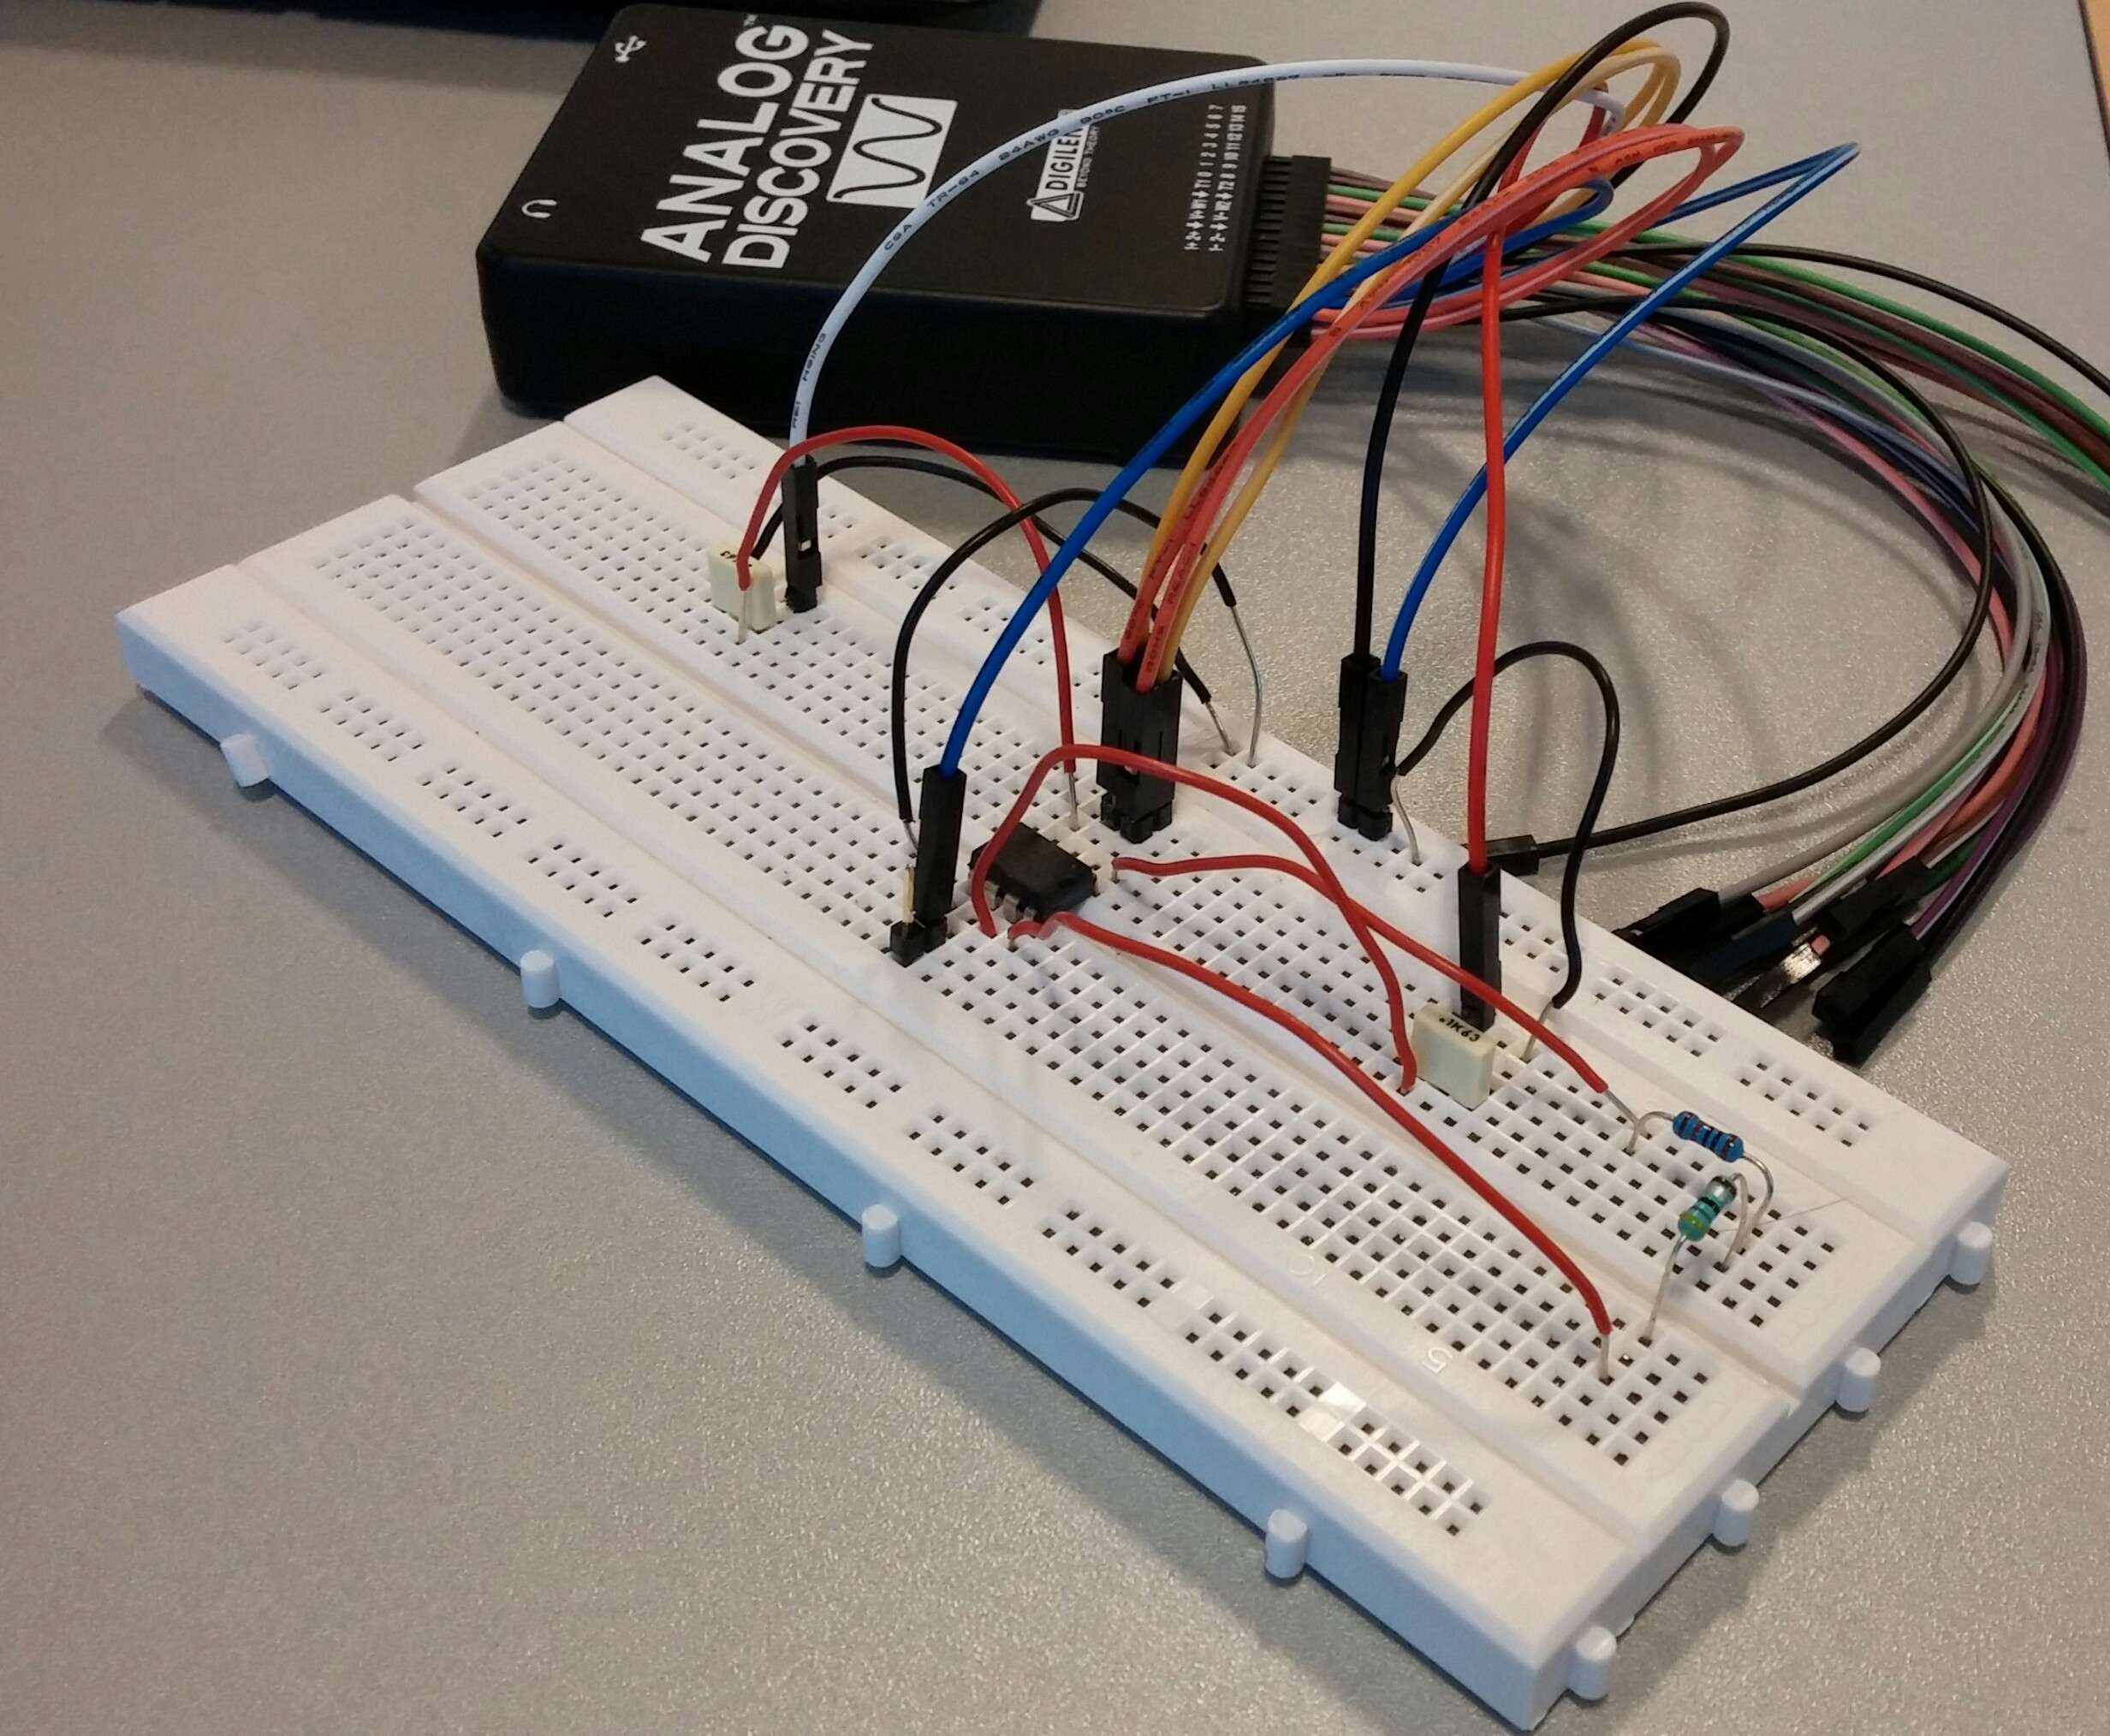
\includegraphics[width=0.7\textwidth]{Figurer/Hardware/ForstaerkerTest}
	\caption{Måleopstilling ved modul test af forstærkeren.}
	\label{fig:ForstaerkerTest}
\end{figure}

Ud af målingerne blev der foretaget lineærregression over de 10 målepunkter. Tendenslinjen der kom ud af den lineæreregression blev som følger:

\begin{figure}[H]
	\centering
	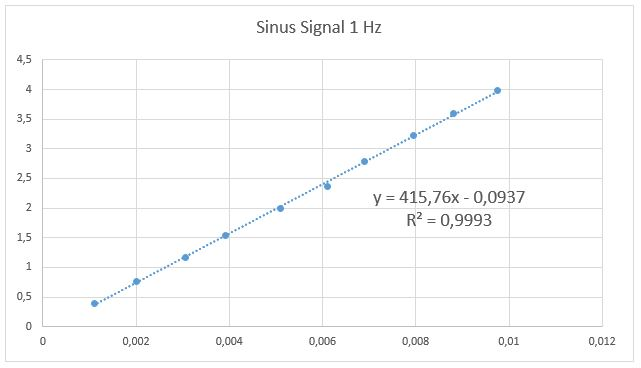
\includegraphics[width=0.7\textwidth]{Figurer/Hardware/Sinusforstaerker}
	\caption{Målpunkter samt tendenslinje for målingerne ved modultest af forstærkeren med 1 Hz sinus-signal.}
	\label{fig:SinusModul}
\end{figure}


I \ref{fig:SinusModul} kan Y beskrives som værende forstærkningen ved en given frekvens. Konstanten 415,8 er den reelle forstærkning som er målt for forstærkeren. Skæringen med y-aksen burde være 0, men grundet måleusikkerheder er den blevet -0,09, hvilket også er acceptabelt. Den høje R$^2$ værdi indikerer, at der er en tydelig lineær sammenhænge mellem den påtrykte spænding og spændingen af output, dvs. forstærkningen er lineær.\\[1ex]
Senere påtryktes samme målopstilling et DC-signal med amplituder startende fra 3mV op til 10 mV. Igen blev amplituden øget med 1 mV for hvert måling således, at der blev 7 målepunkter. Ved målinger foretaget på signaler med både 1 mV og 2 mV er offsettet i Analog Discovery så stort, at målingerne er umulige at fortage.

Forstærkning som blev beregnet på baggrund af de målte output og input viste sig at være meget varierende. Der blev beregnet forstærkninger fra et sted mellem 784 gange og 455 ganges forstærkning. Dets lavere offset jo større forstærkning. Ud fra denne iagttagelse blev det antaget at denne meget store afvigelse måtte skyldes et negativt offset inde i Analog Discovery. 
\\For at finde frem til dette offset blev output spændingen dividerert med 400 som var den ventede forstærkning. Det målte input og resultatet fra den forrrige udregning blev trukket fra hinanden. Heraf sås det at offsettet for Analog Discovery måtte være 12 mV.\\
Dette blev eftertestet med et digitalt multimeter, der rigtig nok målte 12mV højere på indgangen af forstærkeren end det som Analog Discovery målte. 

\begin{figure}[H]
	\centering
	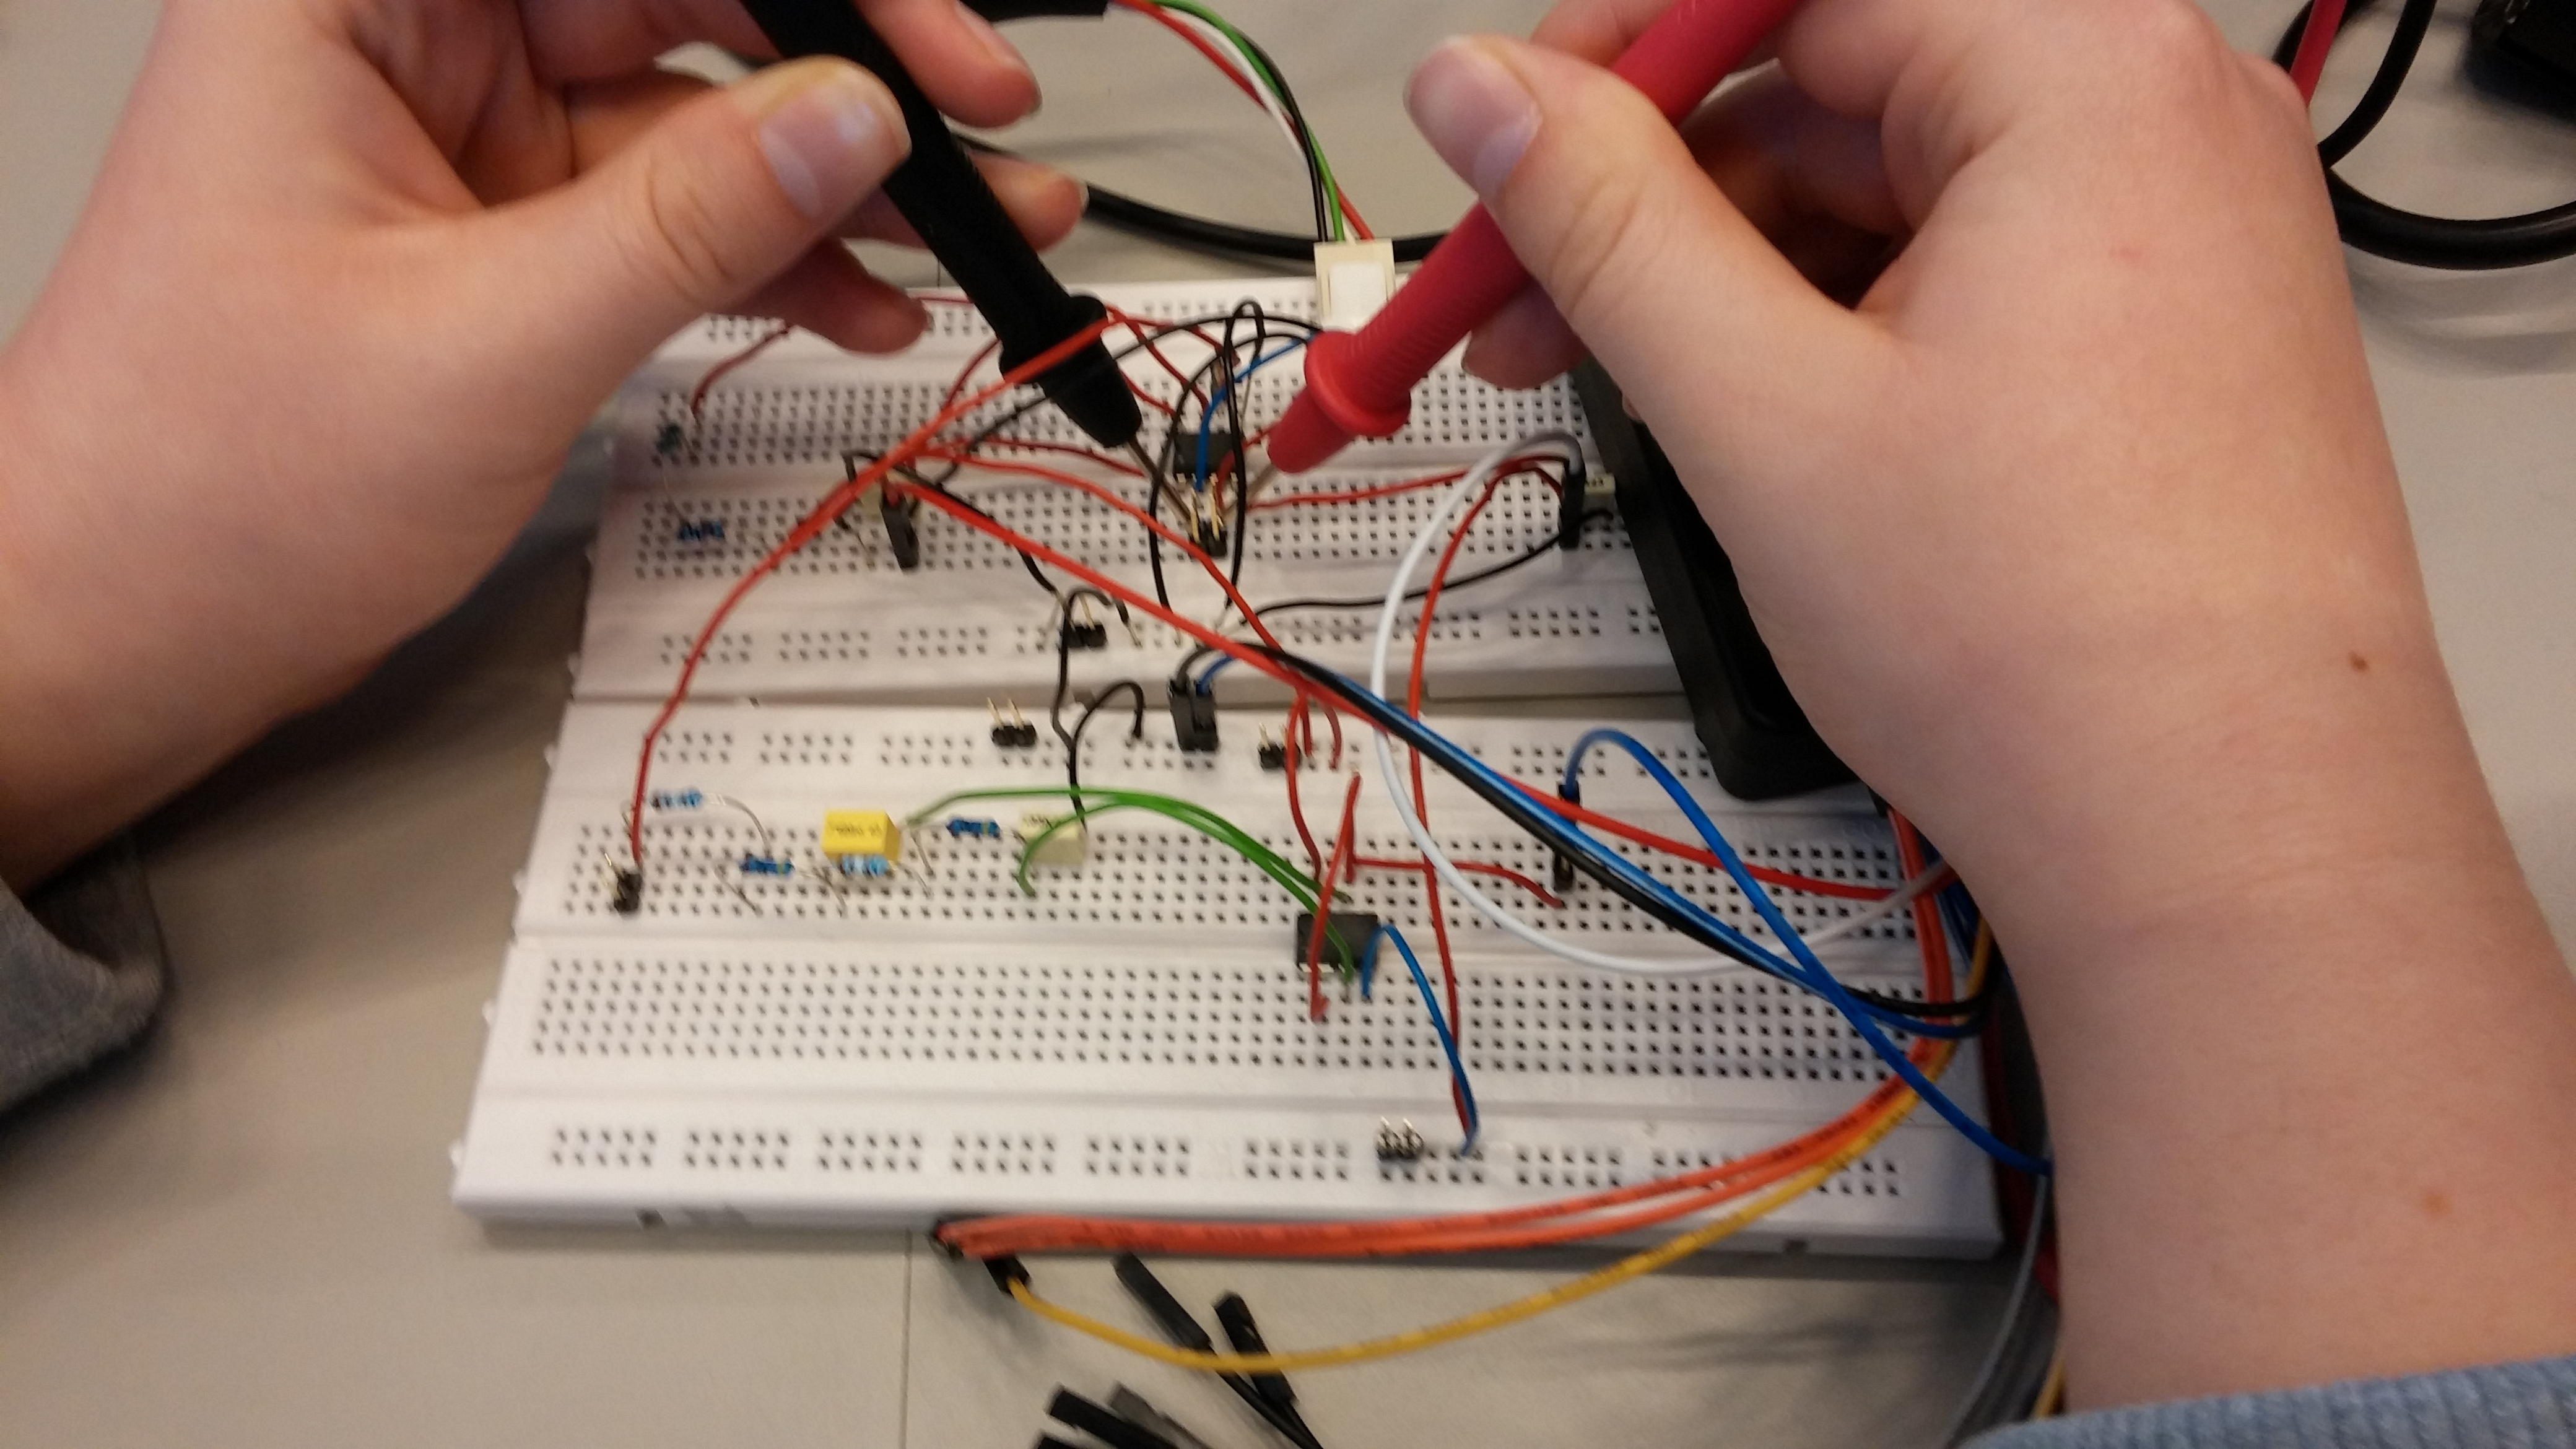
\includegraphics[width=0.7\textwidth]{Figurer/Hardware/DigitalMultimeter}
	\caption{Måling på indgangen af forstærkeren med det digitale multimeter.}
	\label{fig:DigitalMulti}
\end{figure}

Efter at have foretaget lineærregression på de 7 målepunkter så tendenslinjen ud som følger:

\begin{figure}[H]
	\centering
	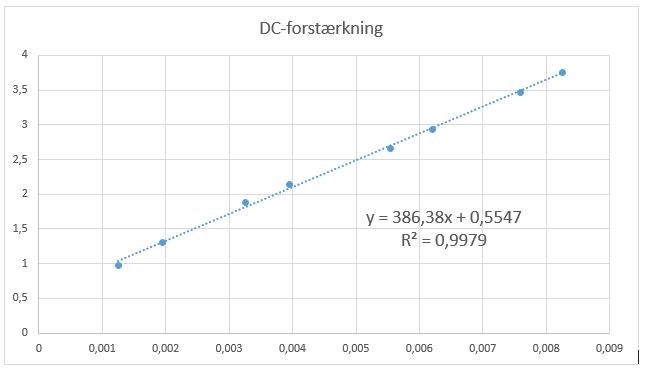
\includegraphics[width=1\textwidth]{Figurer/Hardware/DCforstaerkning}
	\caption{Målpunkter samt tendenslinje for målingerne ved modultest af forstærkeren med DC-signal.}
	\label{fig:DCModul}
\end{figure}

Ud af \ref{fig:DCModul} ses at forstærkningen givet ud fra de 7 måle punkter er på 386 hvilket er en del under den målte forstærkning når systemet påtrykkes et sinussignal i stedet for et DC-signal. Dette kan skyldes at der i målingen af DC-signalet er færre målepunkter, og at det dermed bliver en mere usikker måling, da selv en mindre måleusikkerhed har en større indflydelse på den målte forstærkning.




\subsection{Modul test af det analoge filter}
I modultesten af det analoge filter blev Analog Discovery brugt som spændingsforsyning, signal generator og som oscilloskop til at måle amplituderne for input signalet og output signalet for filteret.

\begin{figure}[H]
	\centering
	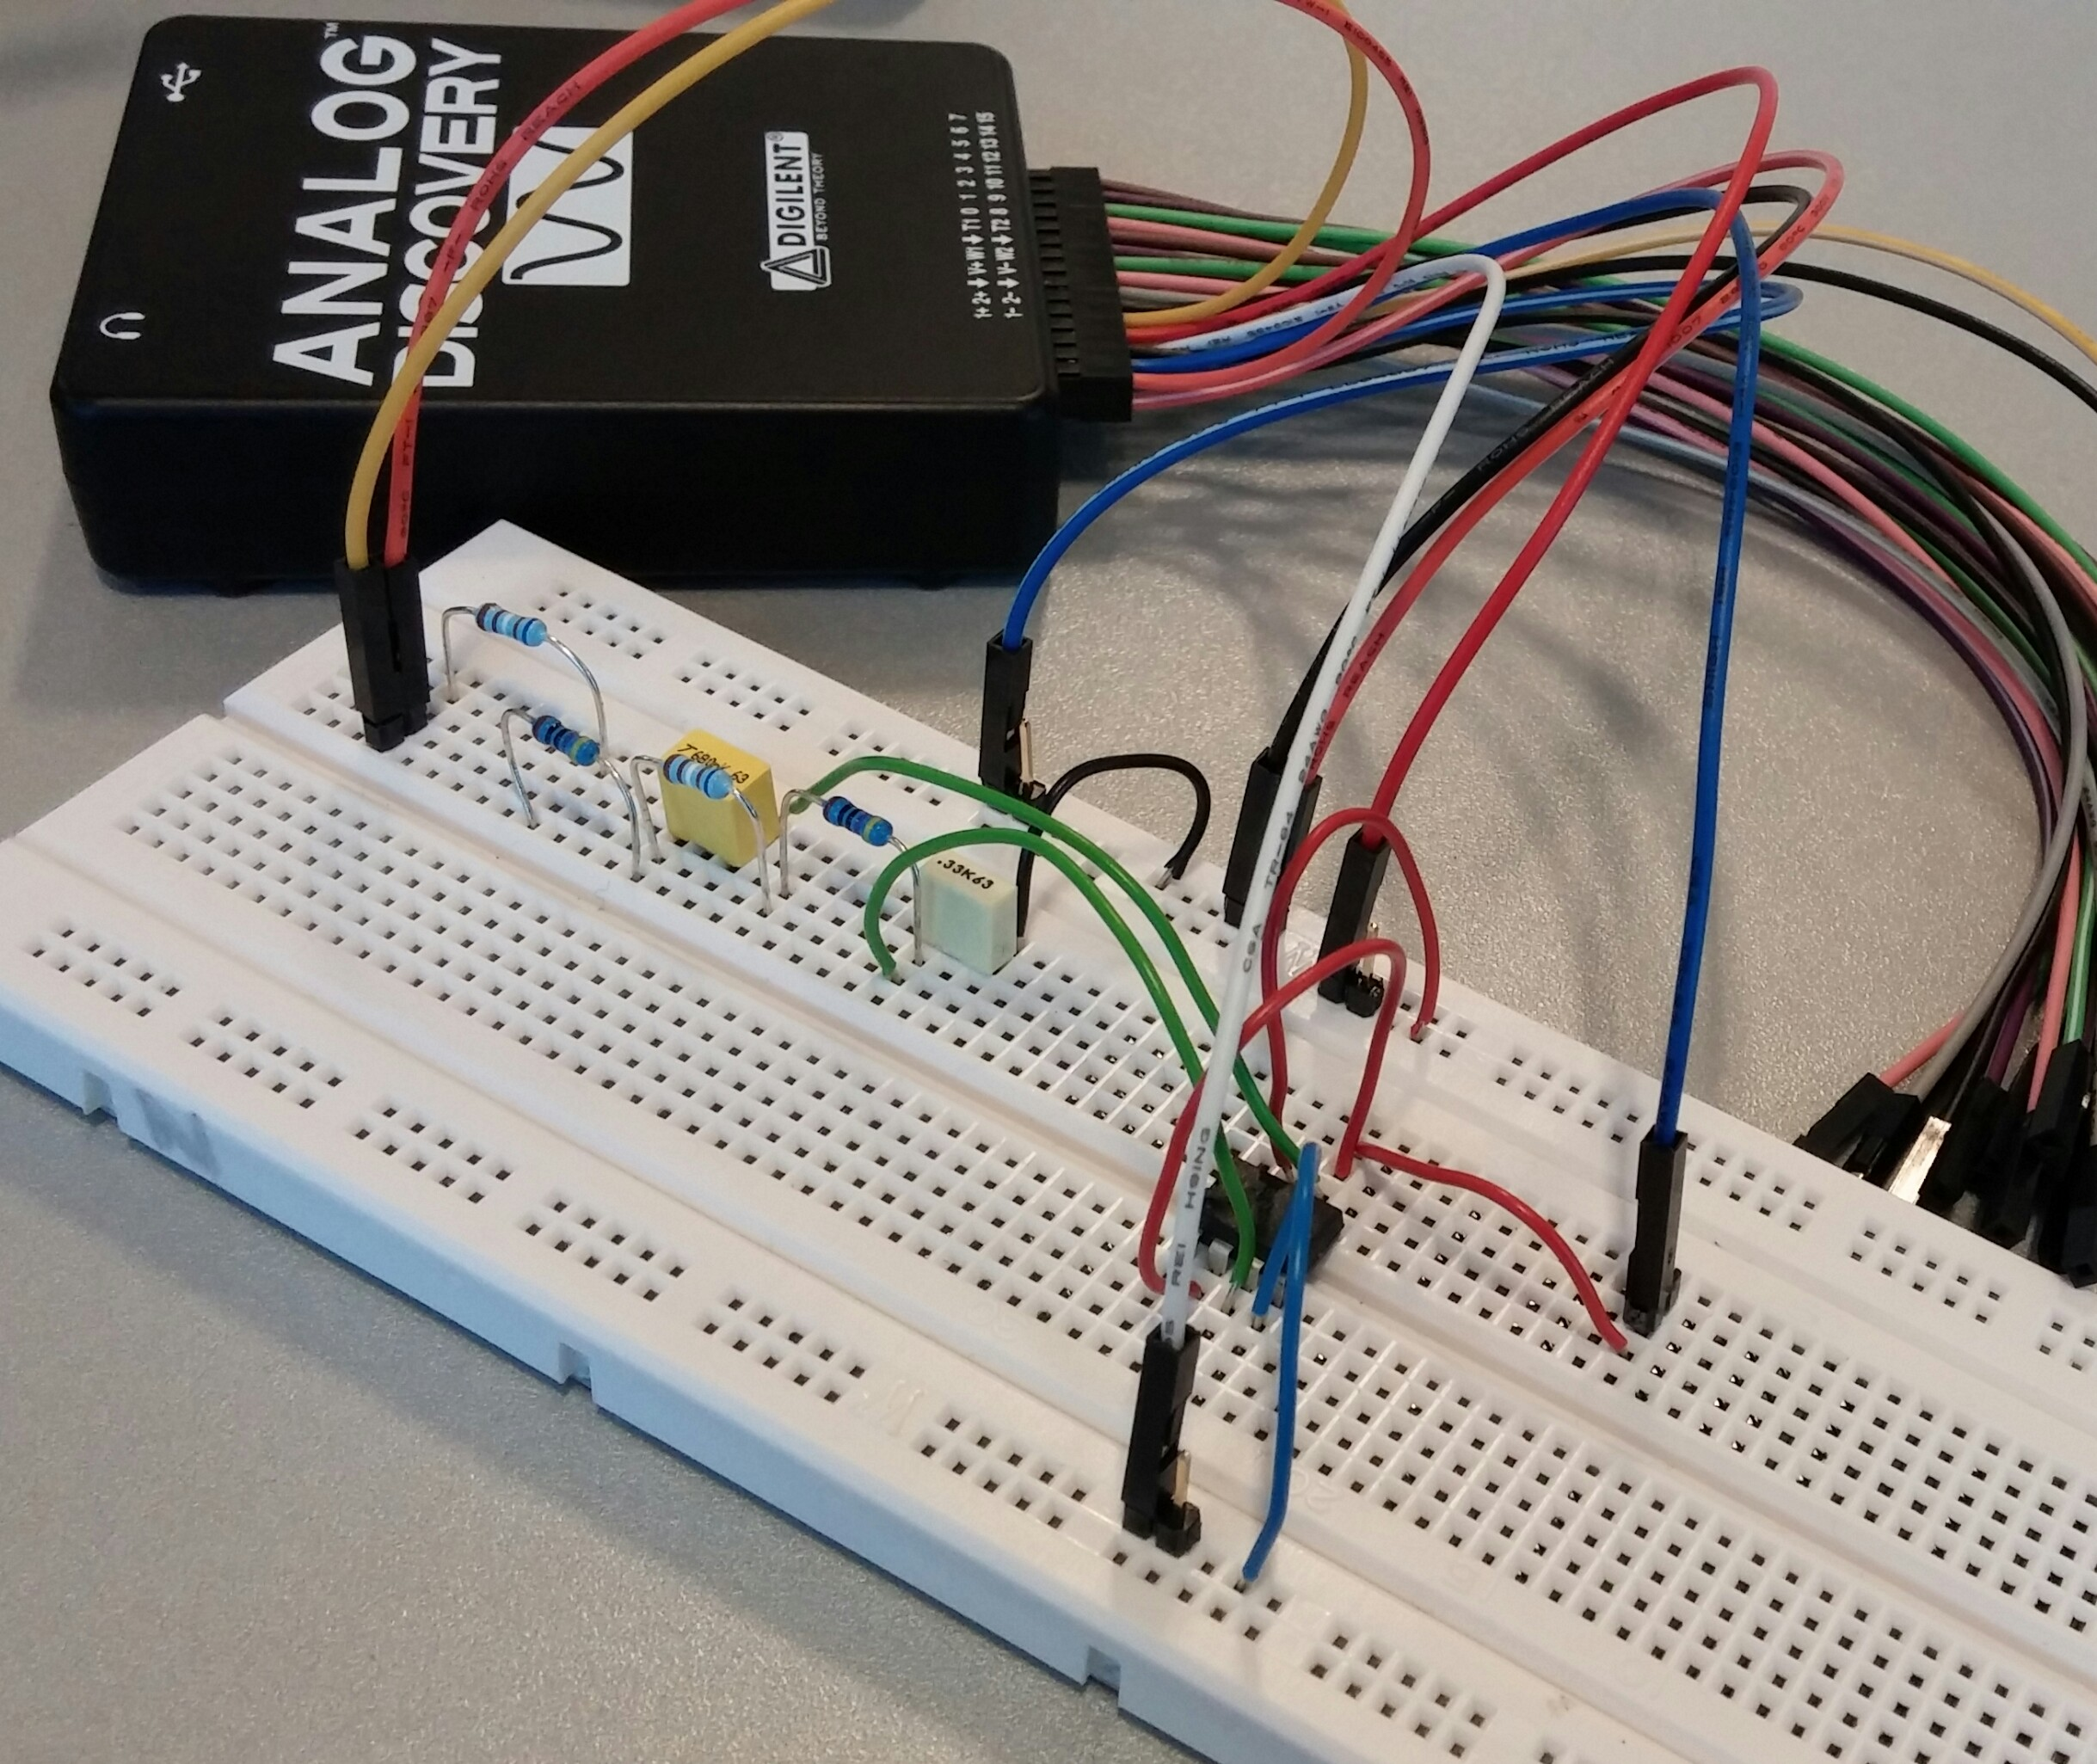
\includegraphics[width=0.5\textwidth]{Figurer/Hardware/FilterTest}
	\caption{Måleopstilling ved modultest af det analoge filter.}
	\label{fig:FilterTest}
\end{figure}

I modultesten af det analoge filter ændres frekvensen for det påtrykte sinussignal på filter indgangen. Der blev målt på i alt 21 målepunkter som lå i intervallet 1 Hz til 500 Hz, se bilag XX for de præcise angivelser af de udvalgte målefrekvenser. Output amplituden samt $\Delta$t mellem de to grafer blev aflæst på de to grafer. På baggrund af disse målinger blev dæmpningen af signalet afbildet. 

\begin{figure}[H]
	\centering
	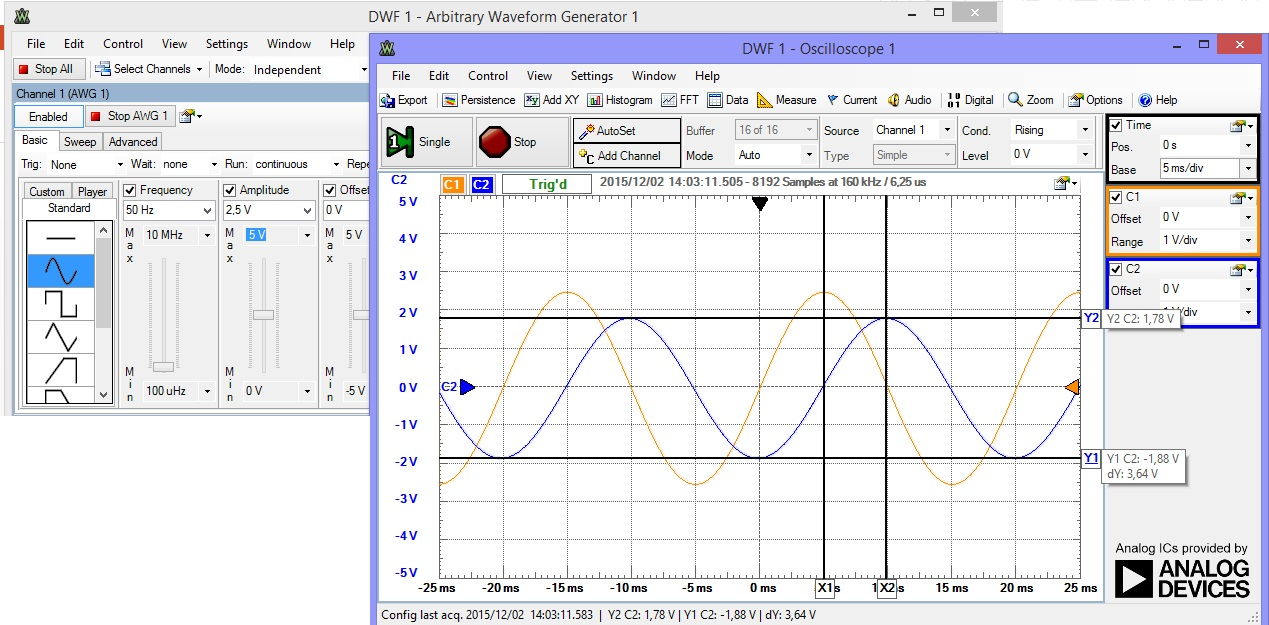
\includegraphics[width=1\textwidth]{Figurer/Hardware/AnalogScreenFilterAmp}
	\caption{Aflæsning af amplitude størrelse for outputsignalet, C2, fra filteret når inputsignalet, C1, har en amplitude på 2,5 V}
	\label{fig:FilterAmplitude}
\end{figure}

Herefter blev tidsforskydningen aflæst således at fasedrejet kunne udregnes.

\begin{figure}[H]
	\centering
	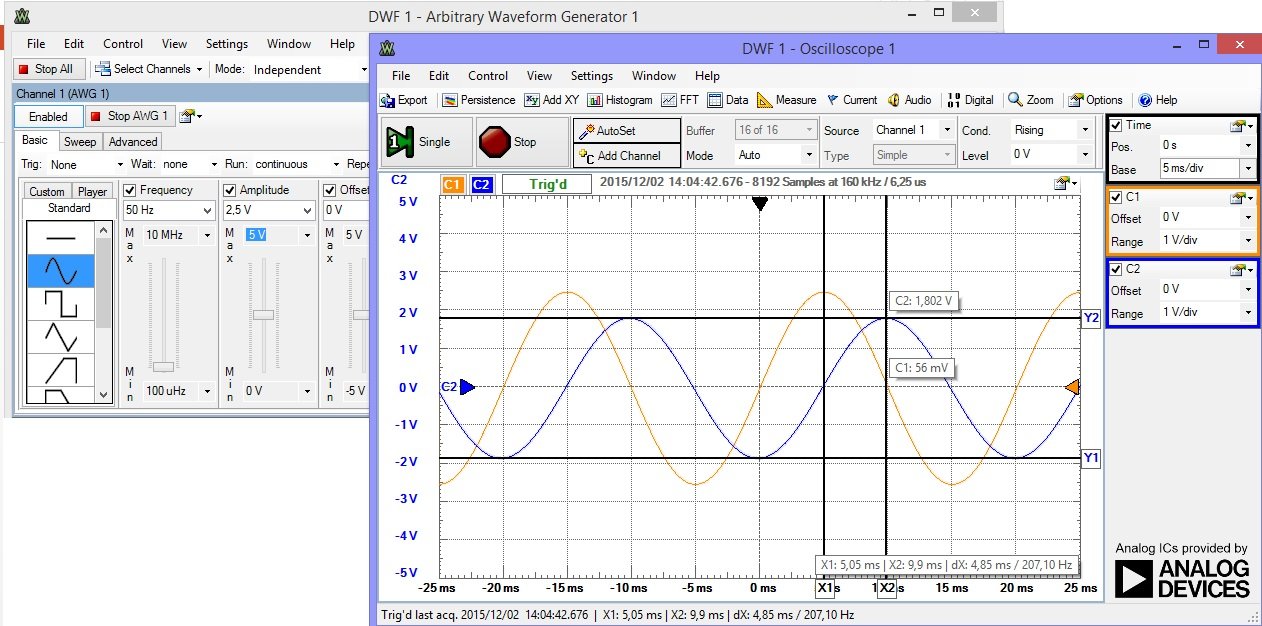
\includegraphics[width=1\textwidth]{Figurer/Hardware/AnalogScreenFilter}
	\caption{Aflæsning af tidsforskydningen for outputsignalet, C2, fra filteret set i forhold til indgangssignalet C1}
	\label{fig:FilterTidsforskydning}
\end{figure}

Det gælder generelt for et 2. ordensfilter af standarttypen som der er arbejdet med igennem projektet, at fasen er 0$^{\circ}$ en dekade før filterets knækfrekvens og falder med -90$^{\circ}$/dekade frem til dekaden efter knækfrekvensen. Derfor skal filteret i praksis have et fasedrej på minus -90$^{\circ}$ ved knækfrekvensen 50 Hz. Som det ses ud graf!! er fasedrejet ved frekvensen 5 Hz -5,2$^{\circ}$, denne skulle reelt set have været 0$^{\circ}$. 
Ved knækfrekvensen som er sat til 50 Hz er fasedrejet -86,4$^{\circ}$, hvor fasedrejet skulle have været -90$^{\circ}$. Ved målingen for 53 Hz er fasedrejet -95,4$^{\circ}$. Dermed kan der argumenteres for, at filterets reelle knækfrekvens må ligge et sted imellem 50 Hz og 53 Hz. 
For målingen på 500 Hz er fasedrejet -180$^{\circ}$, hvilket stemmer overens med teorien for 2. ordensfilterets fasekarakteristik.

\subsection{Integrationstest for forstærker og analogt filter}
Til integrationstesten af forstærkeren og det analoge filter blev Analog Discoverys signalgenerator koblet til indgangen på forstærkeren som blev påtrykt et sinussignal. Filter og forstærker blev koblet sammen således output fra forstærkeren løb over i filterets input. Desuden fungerede Analog Discovery som spændingsforsyning for både forstærkeren og det analoge filter.\\
Der blev udført to målinger for hver udvalgte målefrekvens, hvor amplituden af sinussignalet var henholdsvis 6mV og 7mV. Der blev dermed foretaget 2 målinger for hver af de 16 frekvenser, der lå i intervallet 1Hz til 1 kHz. 

\begin{figure}[H]
	\centering
	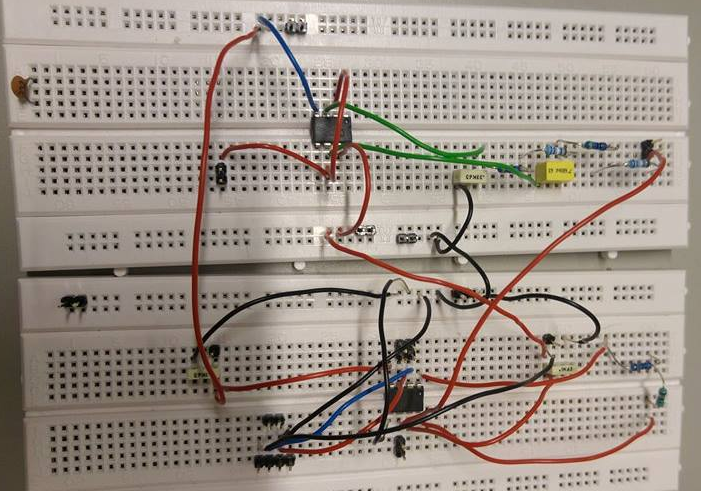
\includegraphics[width=0.7\textwidth]{Figurer/Hardware/samletopstilling}
	\caption{Opstillingen der blev brugt til test af forstærker og analogt filter}
	\label{fig:ForstaerkerFilterOpstiling}
\end{figure}

Da projektet tager udgangspunkt i, at et maksimalt blodtryk vil have en amplitude på 6,25 mV er de to måle amplituder 6mV og 7mV blevet udvalgt for på den måde at kunne eftervise, at forstærkeren og filteret sammen får forstærket signalet op som det skal. Samtidig er de forskellige målefrekvenser udvalgt med henblik på at vise, at signalet på trods af forskellige indgangsamplitude har den samme knækfrekvens, hvilket man kan se ud af \ref{fig:ForstaerkerFilterGraf}.

\begin{figure}[H]
	\centering
	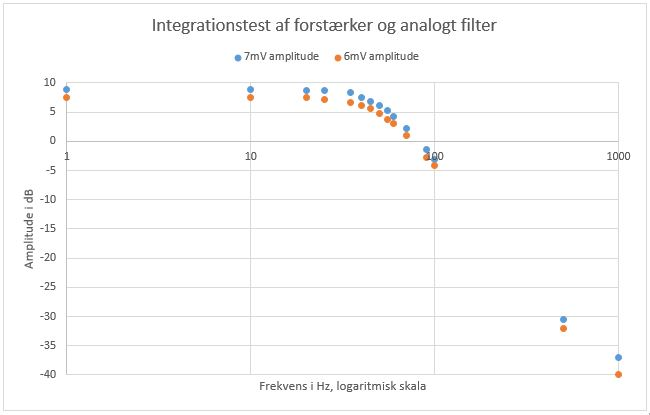
\includegraphics[width=0.7\textwidth]{Figurer/Hardware/IntegrationstestForstaerkerFilter2}
	\caption{Opstillingen der blev brugt til test af forstærker og analogt filter}
	\label{fig:ForstaerkerFilterGraf}
\end{figure}

Som det kan ses ud af \ref{fig:ForstaerkerFilterGraf} viser amplitude karakteristikken for signaler ved hver af de to forskellige amplituder bliver forstærket relativt lige meget dvs. de to amplitude karakteristikker følges ad.
Knækfrekvensen som med de pågældende komponentværdier er udregnet til værende 50,37 Hz \ref{Implementering}. Knæk frekvensen kan findes på grafen ved af aflæse 3dB frekvensen. Denne kan udregnes ved følgende ligning:
\begin{center}
\begin{align}
3dB_{frekvens}=\frac{V_{max}}{\sqrt{2}}
\end{align}
\end{center}
For signalet med amplitude karakterisikken for 7mV bliver 3dB frekvensen dermed som følger:\\
$3dB_{frekvens}=\frac{7mV}{\sqrt{2}}=4,95mV$

Ved aflæsning på grafen kan man ud for ca. 5 mV se, at grafen på x-aksen kan aflæses til at ligge meget tæt på et mål punkt der ligger i data sættet hedder (55 Hz, 5,2 dB), se bilag XX. Ud fra denne oplysning må det antages at den målte knækfrekvens ligger lige en anelse under 55 Hz. Dog er den målte knækfrekvens for systemet højere end 50Hz da forstærkningen ved målingen for 50 Hz er ca. 6 dB.\\
Ud af grafen og det dertilhørende dataset kan det også læses at forstærkningen falder med næsten 40dB/dekade efter knækfrekvensen, med en afvigelse på 3,4 dB.\\
\begin{figure}[H]
	\centering
	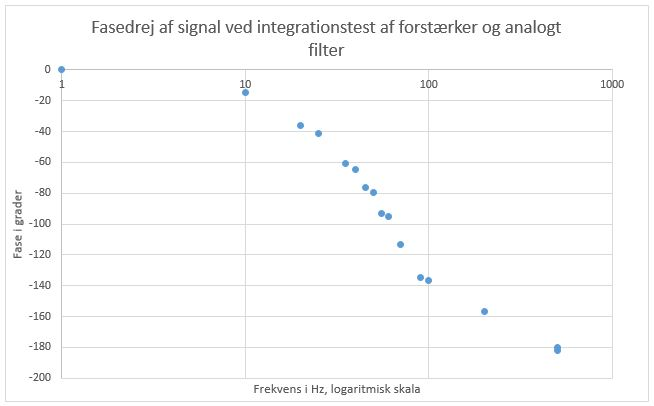
\includegraphics[width=0.7\textwidth]{Figurer/Hardware/FaseForstaerkerFilter}
	\caption{Fasedrej for signalet ved integrationstest af forstærker og analogt filter. Fasedrejet af signalet er målt i grader i forhold til frekvens i Hz.}
	\label{fig:FaseForstaerkerFilter}
\end{figure}
Ud af \ref{fig:FaseForstaerkerFilter} ses det, at filteret og forstærkeren sammensat har et fasedrej på -90$^{\circ}$ ved et sted mellem 50 Hz og 55 Hz. Desuden ses det, at faseforskydningen allerede begynder en dekade før knækfrekvensen og er nede i 180$^{\circ}$ ved ca. en dekade over knækfrekvensen.

\subsection{Integrationstest med vandsøjle}
I integrationstesten med vandsøjlen blev hele hardware delen dvs. transducer, forstærker og analogt filter testet på en vandsøjle, med et bestemt tryk. Transduceren blev koblet til vandsøjlen.\\
\begin{figure}[H]
	\centering
	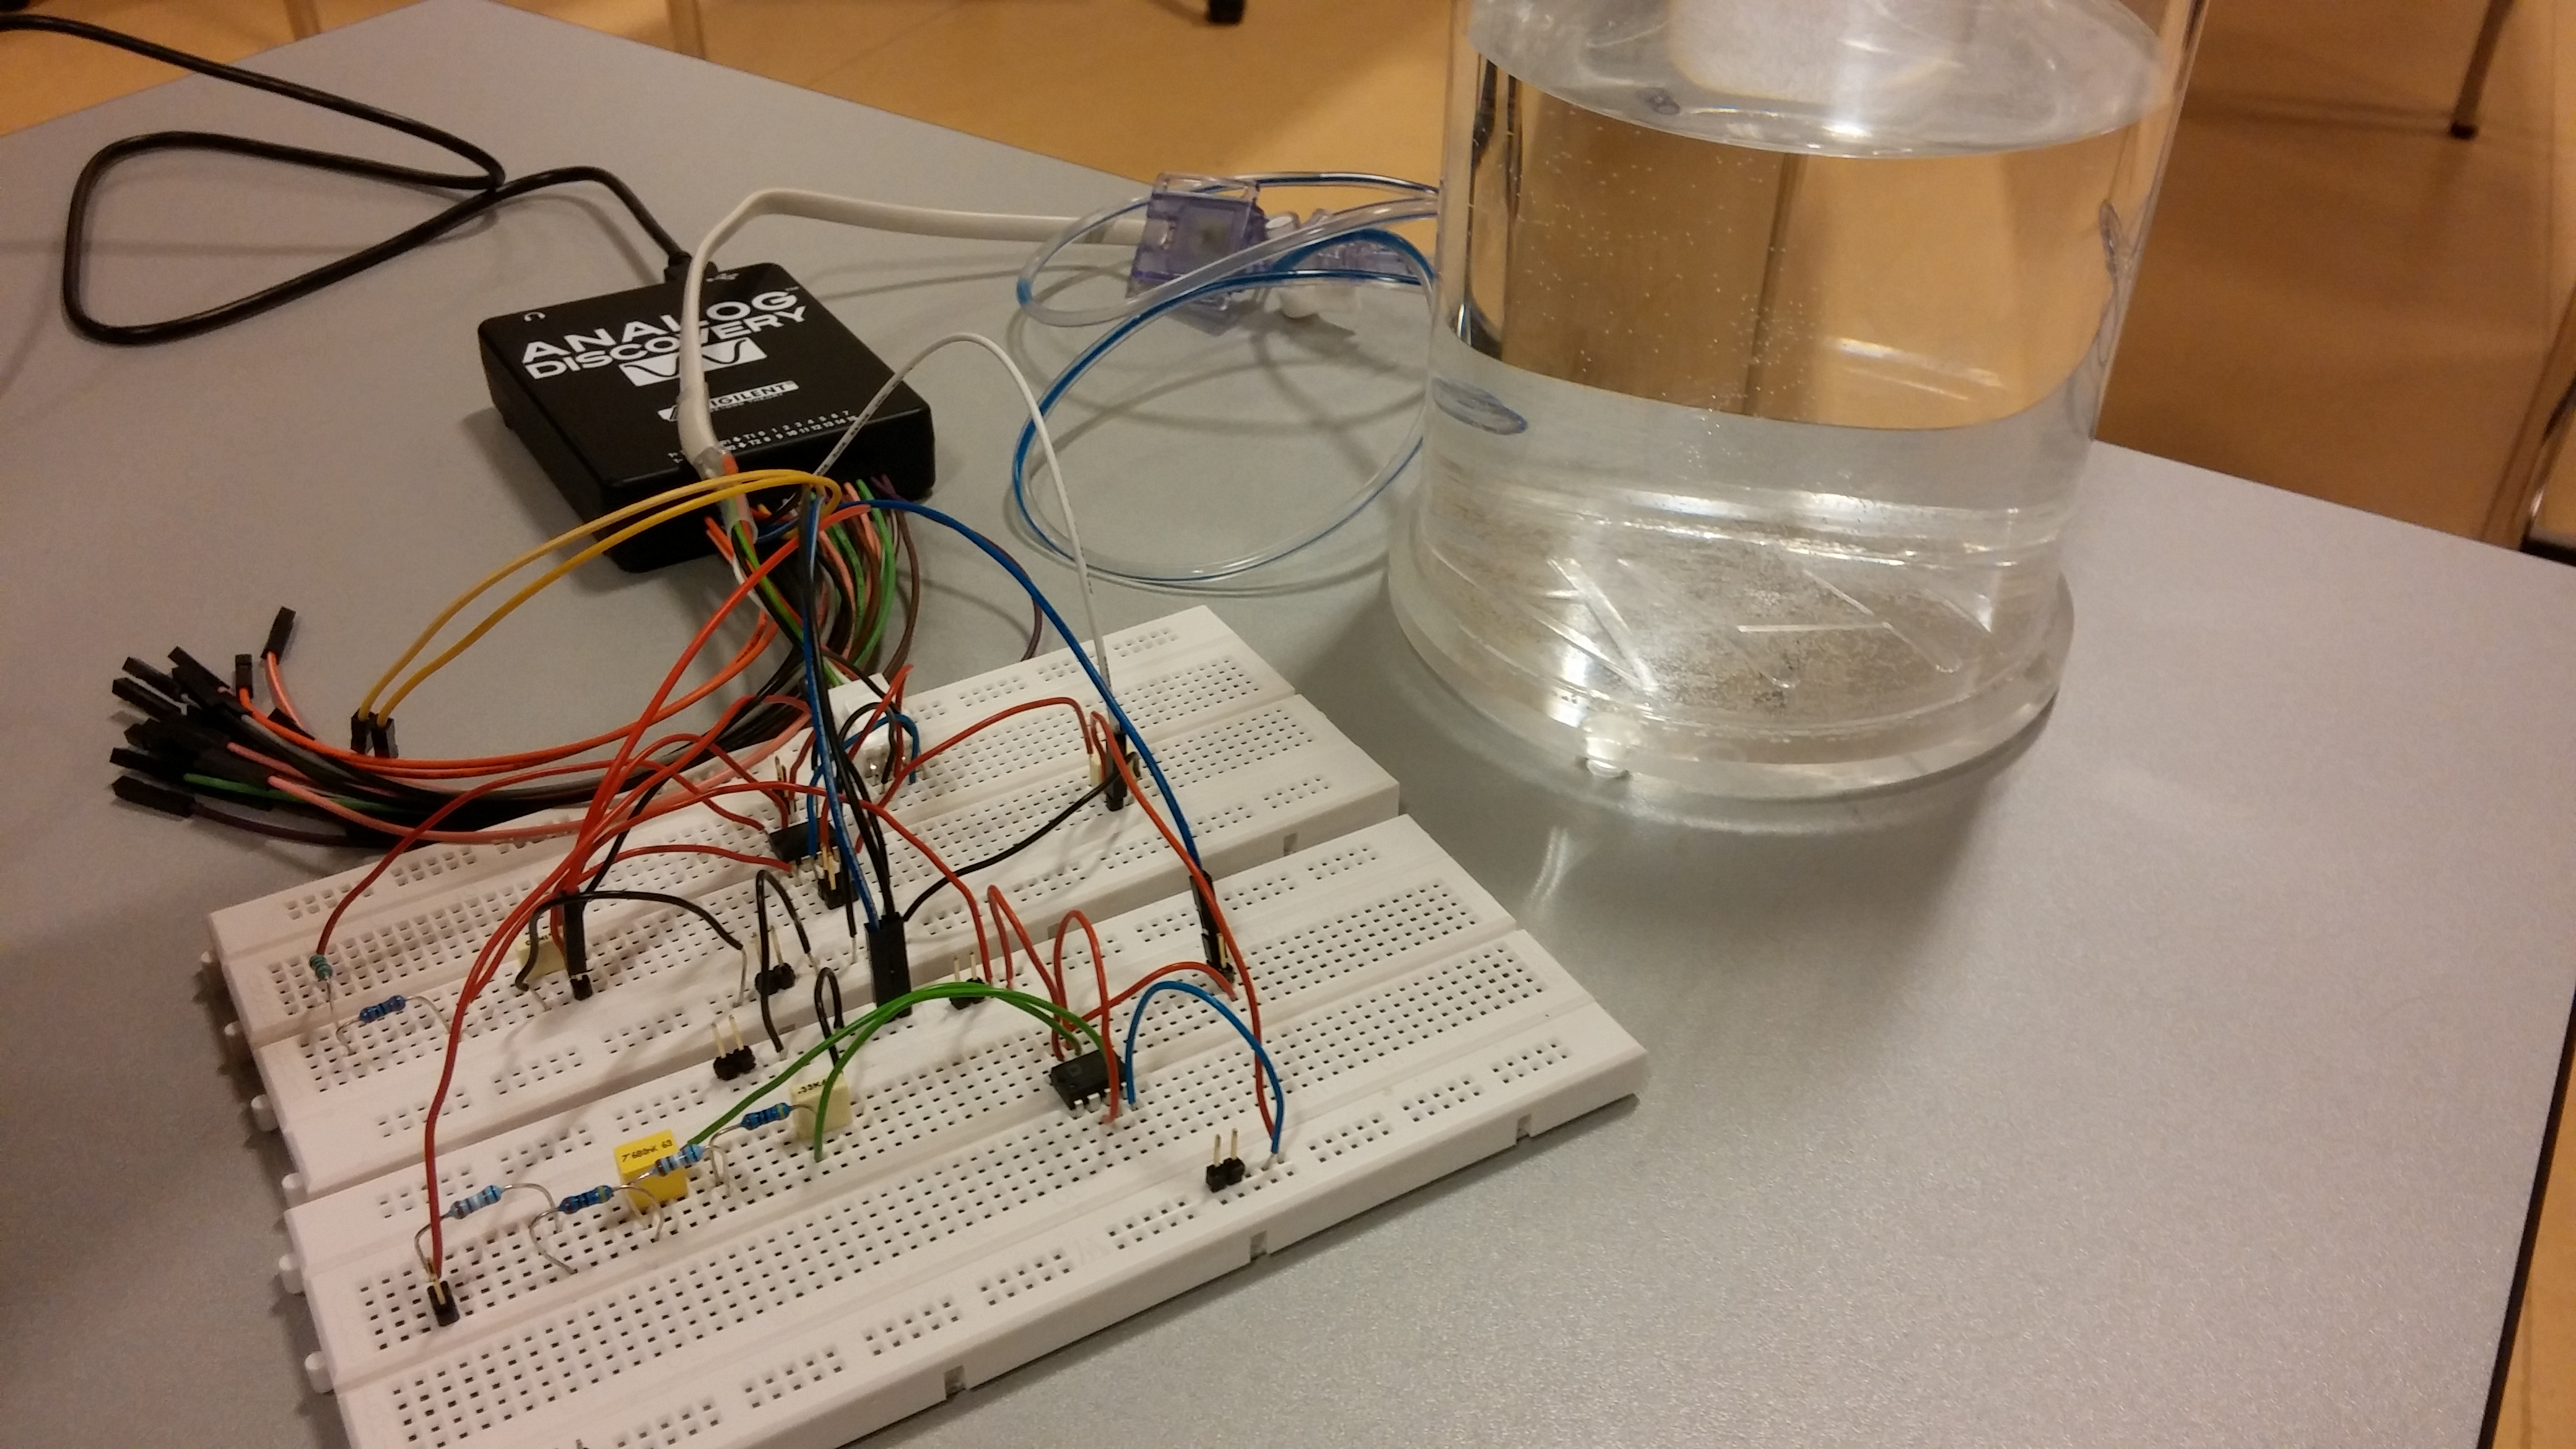
\includegraphics[width=1\textwidth]{Figurer/Hardware/IntegrationVandsoejle}
	\caption{Opstillingen som blev brugt til integrationstest af hardwaredelen med vandsøjle}
	\label{fig:IntegrationVandsoejle}
\end{figure}
Ved det kendte vandsøjletryk i mmHg blev udgangsspændingen for det analoge filter noteret. Efter at have lavet lineær regression over de 5 måle punkter blev tendenslinjens ligning sammenlignet med en tendenslinje, der var lavet på baggrund af 5 teoretisk beregnet punkter. 
\begin{figure}[H]
	\centering
	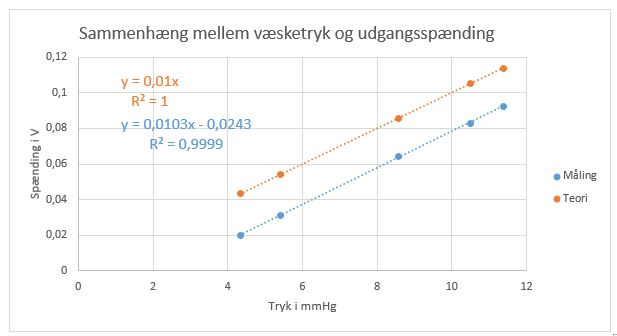
\includegraphics[width=1\textwidth]{Figurer/Hardware/VaesketrykUdgangsspaending}
	\caption{Sammenhængen mellem væsketryk input på indgangen af forstærkeren og udgangsspændingen på filteret. Angivet ved henholdsvis teoretisk beregenet målpunkter og målte punkter.}
	\label{fig:Vaesketryk}
\end{figure}
Ud af \ref{fig:Vaesketryk} ses det, at de to tendenslinjer ligger næsten parallelt faktisk er hældningskoefficienten som er målt på systemet kun 0,0003 større end det er tilfældet for den teoretisk beregnede linje. Dvs. at de to linjer næsten er parallelle. Hvis de to linjer havde været fuldkommen parallelle ville man med sikkerhed kunne sige, hvor stort væsketryk, der er i søjlen på baggrund af det spændings output der er på udgangen af det analoge filter. I systemets tilfælde afviger hældningskoefficienten med 3\% hvilket må siges at være acceptabelt grundet målusikkerheder.


\section{Integrationstest hardware}


\section{Integrationstest software}
I dette afsnit vil der beskrives hvordan systemets dele er blevet testet sammen. Dettet fører videre fra unit testen, hvor de eneklte del elementer blev testes og nu vil disse del elementer blive testet sammen som et helt system. 

\section{Integrationstest system}
I dette afsnit beskrives hvordan software systemet testes sammen med hardware systemet. Denne test forudsætter, at der er lavet integrationstest for både hardware og software hver for sig. \\
Denne integrationstest ligger på til accepttesten som udøfres med kunden. Det er derfor vigtigt at få de to systemer testet sammen inden den endelige accepttest foretages. 
\\
Transduceren kobles til vandsøjlen hvor højden fyldes til 9 cm dvs. et tryk på 6,61 mmHg. Transduceren kobles til hardwaren og der måles på udgangene fra filtret vha. Analog Discovery. Udgangssignalet fra filtret sendes igennem DAQ’en og ind i computeren. Der sættes breakpoints i programmet ved værdien for nulpunktsjustering og værdien af signalet. 
Transduceren sættes til at måle atmosfærisk tryk og der foretages en nulpunktsjustering i programmet. Værdien på Analog Discovery sammenlignes med værdien der ses i koden. Her ses at der kun er en forskel på 2,1 mV hvilket kan skyldes at signalet svinger lidt da trykket ikke er helt jævnt. 

\begin{figure}[H]
	\centering
	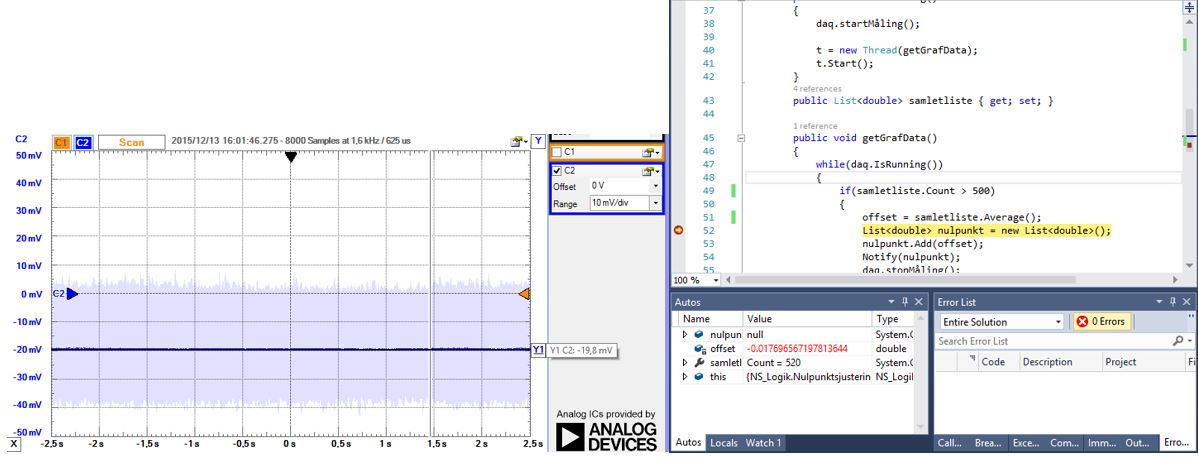
\includegraphics[width=1.2\textwidth]{Figurer/Test/Nulpunkt}
	\caption{Værdien fra det atmosfæriske tryk målt med Analog Discovery til -19,8 mV (til venstre) og med programmet til -0,0177 V (til højre).}
	\label{fig:Atmosfaerisktryk}
\end{figure}

Transduceren sættes til at måle trykket fra vandsøjlen. Dernæst foretages en måling i programmet. I selve koden findes værdien der måles og denne sammenlignes med målingen i Analog Discovery. Her ses at signalet programmet opfanger svinger omkring værdien vi måler med Analog Discovery. Dette kan skyldes at vandsøjlens overflade står og vibrere med rystelserne i bordet, hvorved der skabes svingninger i signalet.

\begin{figure}[H]
	\centering
	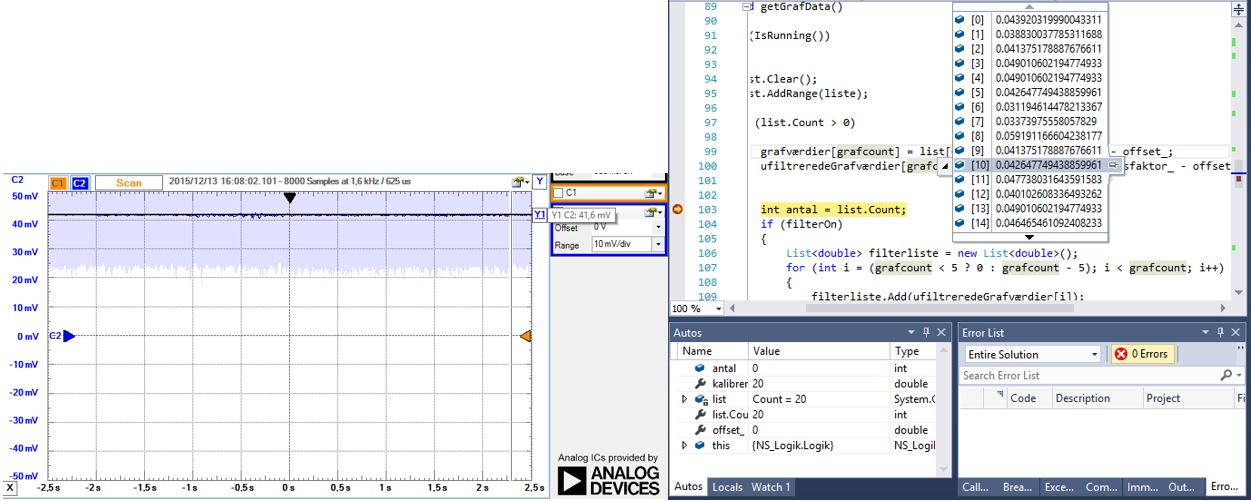
\includegraphics[width=1.1\textwidth]{Figurer/Test/Vandsoejle}
	\caption{Værdien fra væsketrykket målt med Analog Discovery til 41,6 mV (til venstre) og med programmet i V (til højre).}
	\label{fig:Vaesketryk2}
\end{figure}

Dernæst sammenlignes det kendte tryk med værdien der vises i programmet. Her ses at værdien af mmHg i programmet ligger lidt under det tryk vi forventer der er i vandsøjlen. Dette kan skyldes måleusikkerheder fra målingen af vandsøjlens højde og ændringen af signalet undervejs i hardwaren og DAQ’en. Svingningerne af værdien i signalet skyldes stadig at vandsøjlens overflade vibrere når der er små vibrationer i bordet vandsøjlen står på.  

\begin{figure}[H]
	\centering
	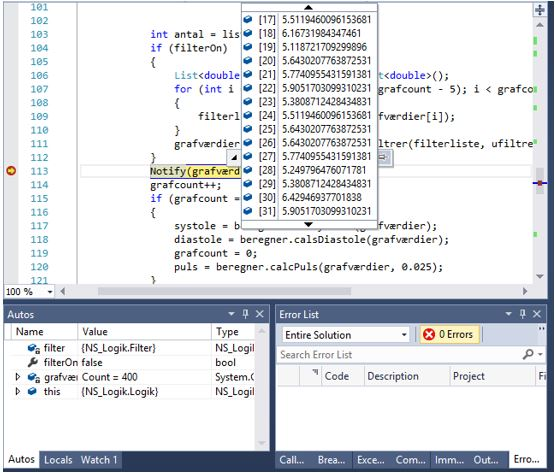
\includegraphics[width=0.6\textwidth]{Figurer/Test/mmHg}
	\caption{Værdien fra Væsketrykket målt med programmet i mmHg.}
	\label{fig:mmHgtryk}
\end{figure}